\documentclass{RITA}
\usepackage{graphicx,url}
\usepackage{subfigure}
%\usepackage[brazil]{babel}   
\usepackage[latin1]{inputenc}  
\usepackage{amsfonts}
\usepackage{amsmath}

\author{
  Anderson Rocha Tavares\footnote{Instituto de Inform\'atica, UFRGS, Caixa Postal~15064\\
  \texttt{\{artavares,bazzan@inf.ufrgs.br\}}}
  \and Ana Lucia Cetertich Bazzan\footnotemark[1]
}

\title{Independent learners in abstract traffic scenarios}

\RITAvolume{XIX}
\RITAnumber{1}
\RITAyear{2012}
\usepackage{graphicx,url}

%\usepackage[brazil]{babel}   
\usepackage[latin1]{inputenc}  
\usepackage{amsfonts}
\usepackage{amsmath}
\usepackage{subfigure}
%\usepackage{algpseudocode}
%\usepackage{algorithm}
     

% Equation terms definition
\newcommand{\route}[1]{\ensuremath{P_#1}}	%route for driver 'i'
\newcommand{\optRoute}[1]{\ensuremath{P_#1^*}}	%optimal route for driver 'i'

\newcommand{\travTime}{\ensuremath{t_j}} 	%travel time on link 'j'
\newcommand{\fftt}{\ensuremath{f_j}} 		%free-flow travel time of link 'j'
\newcommand{\linkCap}{\ensuremath{c_j}}		%capacity of link 'j'
\newcommand{\veh}{\ensuremath{v}}		%number of vehicles

\newcommand{\ett}[1]{\ensuremath{e_#1}}		%estimated travel time for agent 'i'
\newcommand{\expVeh}{\ensuremath{v_e}}		%estimated number of vehicles

\newcommand{\att}[1]{\ensuremath{u_#1}}		%actual travel time for driver 'i' on route P

\newcommand{\reward}[1][]{\ensuremath{R_#1}}	%reward

\newcommand{\congRoads}{\ensuremath{C}}		%the set of congested roads
\newcommand{\numCong}{\ensuremath{n}}		%number of congested roads
\newcommand{\overLoadFactor}{\ensuremath{o}}	%overload factor - measures severity of congestions



\begin{document}

\maketitle

\begin{abstract}
Traffic is a phenomena that emerges from individual, uncoordinated and, most of the times, selfish route choice made by drivers. This work presents a reinforcement learning based approach for route choice which relies solely on drivers experience to guide their decisions. There is no coordinated learning mechanism, so that driver agents are independent learners. Our approach is tested on two abstract traffic networks and it is compared to other route choice methods. Experimental results shows good performance regarding travel times and road network load balance. The simplicity, realistic assumptions and performance of the proposed approach makes it feasible of being implemented on navigation systems.
\end{abstract}


%\category{I.2.11}{Artificial Intelligence}{Distributed Artificial Intelligence}[Multiagent Systems]

%\terms{Algorithms}

%\keywords{Multiagent reinforcement learning, multiagent systems, traffic assignment}

\section{Introduction}
\label{sec:intro}

Traffic and mobility present challenging issues to authorities, traffic engineers and researchers. To deal with the increasing traffic demand, techniques and methods to optimize the existing road traffic network are attractive since they do not include expensive and environmental-impacting changes on the infrastructure.

In a commuting scenario, it is reasonable to assume that drivers choose their routes independently and, most of the time, uninformed about real-time road traffic condition, thus relying on their own experience. Daily commuters usually have an expectation on the time needed to arrive on their destinations and, if a driver reaches its destination within that expectation, his travel time can be considered  reasonable. From a global point of view, it is desired that vehicles gets distributed on the road network proportionally to the capacity of each road. In a commuting scenario, drivers strive to minimize their travel times. At the same time, there is an global cost function which rates the whole system's behavior, like distribution of vehicles in proportion to the capacity of each road. Multiagent systems such as this commuting scenario are called collectives. The local and global goals can be highly conflicting and there is no general approach to tackle this complex question of collectives, as shown by Tumer and Wolpert \cite{Tumer&Wolpert2004}.

Traffic assignment deals with route choice between origin-destination pairs in transportation networks. In this work, traffic assignment will be modeled as a reinforcement learning problem so that agents make decisions using only their own experience, which is gained through interaction with the environment. The environment is a road network that abstracts some real-world characteristics such as vehicle movement along the roads, allowing us to focus on the main subject which is the choice of one route among the ones available for each driver.

The remainder of this document is organized as follows: Section \ref{sec:concepts} presents basic traffic engineering, single and multiagent reinforcement learning concepts that will be used throughout this paper. Section \ref{sec:related} presents and discusses related works. Section \ref{sec:proposal} presents the reinforcement learning for route choice approach, whose results are discussed in Section \ref{sec:results}. Finally, Section \ref{sec:conclusions} concludes the paper and presents opportunities for further investigation.

\section{Background}
\label{sec:concepts}
\subsection{Commuting and traffic flow}

A road network can be modeled as a graph, where there is a set of nodes, which represent the intersections, and links among these nodes, which represent the roads. The weight of a link represents a form of cost associated with the link. For instance, the cost can be the travel time, fuel spent or length.

A subset of the nodes contains the origins of the road network, where drivers start their trips, while another subset represents the destinations. In a commuting scenario, a driver's trip consists on a set of links, forming a route between his origin and destination (OD pair) among the available routes.

Traffic flow is defined by the number of entities that use a network link in a given period of time. Capacity is understood as the number of traffic units that a link supports in a given instant of time. Load is understood as the demand generated on a link at a given moment. When demand reaches the link's maximum capacity, congestion is formed.

Traffic assignment methods that consider congestion effects in urban settings need a suitable cost function that relates link's attributes (capacity, free-flow travel time) and traffic flow on the entire road network. However, a simplified form that relates attributes of a  given link and traffic flow only on that link can be used, although with some loss of realism. One of the most common function of this type is shown on Eq. \eqref{eq:tt} \cite{Ortuzar&Willumsen2001}.

\begin{equation}
\label{eq:tt}
\travTime(\veh) = \fftt[1 + \tau \left(\frac{\veh}{\linkCap}\right)^\beta]
\end{equation}

In this function, $\travTime$ is the travel time on link $j$, $\linkCap$ is the link's capacity, $\fftt$ is the free-flow travel time on link $j$ and $\tau$ and $\beta$ are calibration parameters. This will be the travel time function used throughout the present work.

\subsection{Reinforcement Learning}
\label{sec:rl}
Reinforcement learning (RL) deals with the problem of making an agent learn a behavior by interaction with the environment. Usually, a reinforcement learning problem is modeled as a Markov Decision Process (MDP), which consists of a discrete set of environment states $(S)$, a discrete set of actions $(A)$, a state transition function ($T: S \times A \to \Pi(S))$, where $\Pi(S)$ is a probability distribution over S) and a reward function $(R: S \times A \to \mathbb{R})$. %$T(s, a, s')$ means the probability to go from state $s$ to $s'$ after performing action $a$ in $s$.

The agent interacts with the environment following a policy $\pi$ and tries to learn the optimal policy $\pi^*$ that maps the current environment state $s \in S$ to an action $a \in A$ in a way that the future reward is maximized. At each state, the agent must select an action $a$ according to a strategy that balances exploration (gain of knowledge) and exploitation (use of knowledge). One of the strategies is $\epsilon$-greedy, that consists on choosing a random action (exploration) with probability $\epsilon$ or choosing the best action (exploitation) with probability $1 - \epsilon$. In the beginning, $\epsilon$ starts with a higher value (high exploration) and decreases with time, leading to high exploitation in the end.

Q-learning is an algorithm that converges towards the optimal policy, given certain conditions \cite{Watkins&Dayan1992}. Its update rule is shown in Eq. \eqref{eq:qlearning}, where $<s,a,s',R>$ is an experience tuple, meaning that the agent performed action $a$ in state $s$, reaching state $s'$, receiving reward $R$. Action $a'$ is one that can be taken on $s'$, $\alpha$ is the learning rate and $\gamma$ is the discount factor. $Q(s,a)$ is an entry indexed by state $s$ and action $a$ in the Q-table, which stores the values (called Q-values) of state-action pairs. The Q-value is the expected discounted reward for executing action $a$ at
state $s$ and following the policy $\pi$ thereafter.

\begin{equation}
\label{eq:qlearning}
Q(s,a) = (1 - \alpha) Q(s,a) + \alpha (R + \gamma \max_{\substack{a'}}(Q(s',a')))
\end{equation}

For a complete description of Q-learning, the reader may refer to \cite{Watkins&Dayan1992}.


%For the next sections it will be assumed that the reader is familiar with Q-learning. For more information about Q-learning, the reader may refer to \cite{Watkins&Dayan1992}.

\subsection{Independent learners} 
Traffic scenarios are associated with the class of non-cooperative multi-agent systems, as there are several agents interacting with the environment and sometimes coordinating themselves to use the traffic network resources. Multi-agent reinforcement learning (MARL) can be divided in two classes: independent learners (ILs), in which agents ignore the existance of other agents, and joint action learners (JALs), in which agents learn the value of their own actions combined with other agents' actions via integration of RL with coordination learning methods \cite{Claus&Boutilier1998}. 

For an independent learner agent, the other agents learning and changing their behavior is understood as a change of environment dynamics. In the present work, agents will be modeled as ILs, because modeling agents as JALs leads to scalability problems, as agents must consider every other agents' actions. 

In complex scenarios like transportation systems, there is a large number of agents, making the modeling of JALs unfeasible. On the other hand, when agents are modeled as ILs, the convergence properties of Q-learning become invalid, as the environment is nonstationary. Also, it is remarked by Littman \cite{Littman1994} that training adaptive agents without considering other agents adaptation is not mathematically justified and it is prone to reaching a local maximum where agents quickly stop learning. Despite this, some researchers achieved amazing results with this approach as Littman \cite{Littman1994} also remarks.

One example of successful application of independent learners can be found on \cite{Tesauro1994}, where the author presents an automated player that uses the TD($\lambda$) reinforcement learning algorithm \cite{Sutton1988} to teach itself to play backgammon. From zero knowledge in the beginning of learning, the automated player learns to play at a strong intermediate level. The automated player reaches strong master level if some prior knowledge is programmed in it. 

Another example of successful application of independent learners can be found on \cite{Crites&Barto1998} where the authors program each member of an elevator car controller team as an independent learner. Results show that the presented approach surpasses the best heuristic elevator control algorithms of that time.

%A multiagent system can be understood as group of agents that interact with each other besides perceiving and acting in the environment they are situated. The behavior of these agents can be designed a priori. In some scenarios this is a difficult task or this pre-programmed behavior is undesired, so that the adoption of learning (or adapting) agents is a feasible alternative \cite{Busoniu+2008smc}.



\section{Related work}
\label{sec:related}

%In traffic engineering, \cite{Bazzan&Kluegl2007} remarks that agent-based simulation is a suitable approach, as agents can be modeled to deal with incomplete information and adapt to dynamic environments. Application of intelligent agent architectures to route choice is present on a number of publications. Next, some works based on this agent-based approach are reviewed.

%Several works, such as \cite{Bazzan+2000icmas,Chmura&Pitz2007,Kluegl&Bazzan2004}, use abstract scenarios, most of the times inspired by congestion or minority games. On these scenarios, agents have to decide between two routes and receive a reward based on the occupancy of the chosen route. This process is repeated and there is a learning or adaptation mechanism that guides the next choice based on previous rewards.

%With this process, a Pareto-efficient distribution or the Wardrop's equilibrium \cite{Wardrop1952} may be reached. In this condition, no agent can reduce its costs by switching routes without rising costs for other agents. 

Traffic assignment problems can be addressed by several approaches, many of them considering abstract traffic scenarios. Two-route scenarios are studied in \cite{Bazzan+2000icmas,Kluegl&Bazzan2004}. The former analyses the effect of different strategies on minority game for binary route choice. The latter includes a forecast phase for letting agents know the decision of the others and then let they change their original decision or not. Each one of these works assessed relevant aspects of agents decision-making process, even though only binary route choice scenarios were studied. The interest on the present work is to evaluate a route choice approach in a more complex scenario, with several available routes.

This kind of complex scenario was investigated by \cite{Bazzan&Kluegl2008}. In their work, Bazzan and Kl\"ugl assessed the effect of real time information on drivers' route replanning, including studies with adaptive traffic lights. In the most successful en-route replanning strategy presented on that work, the authors assume that the entire network occupancy is known by the drivers. This assumption was needed for assessing the effects of re-routing, although the availability of real time information of the entire network for all the drivers is an unrealistic assumption.

%More recently, Galib and Moser \cite{Galib&Moser2011} proposed a modified version of the minority game for use in a complex scenario with several available routes. 
The problem of traffic assignment can also be tackled by an evolutionary game called minority game \cite{Challet&Zhang1997}. In evolutionary games, it is assumed that players (or agents) have bounded rationality and use inductive reasoning to make their decisions. This is suitable to the transportation domain as humans do have bounded rationality and inductive reasoning is used in human decision-making process, as remarked by Arthur \cite{Arthur1994}.

The minority game consists of an odd number of player agents that must choose between two options at each round. Agents on the minority side receive one point. The only information available for agents is the history of winning options. Each agent has a set of strategies that predicts the next winning option given the history. Agents score each strategy according to the number of times it went correct and they use the best strategy to make the prediction for the next round.

Regarding the traffic assignment problem, the minority game can only be used in two-route choice scenarios as it is a two-alternative game. To overcome this limitation, Galib and Moser \cite{Galib&Moser2011} proposed a modified version of the minority game for a complex scenario with several available routes. In this modified version, agents' strategies predict a road's occupancy given the occupancy history on the past trips. Using the proposed approach, drivers achieve reasonable (within expectation) travel times and distribute themselves over the road network in a way that few links get overused. The proposed approach uses historic usage data of all links to choose the next one on the route. Having historical information of the links used by the driver is a reasonable assumption, but having historic information of all links on the network is unrealistic. The approach proposed on the present work will be compared with the modified minority game. 

%TODO cut other IL works???%%% Prior to the present work, independent learning agents were studied in cooperative repeated games \cite{Claus&Boutilier1998,Tan1993,Sen+1994}. The present study is an application of the independent learners concept in a competitive multi-agent system as agents compete for a resource (the road network). Decisions on this route choice scenario are sequential, making this a more complex scenario.

Learning-based models for route choice are studied in \cite{Chmura&Pitz2007,Ben-Elia&Shiftan2010}. In the former, the authors present a reinforcement algorithm and in the latter, a reinforcement-based model of route-choice behavior with availability of real-time information is presented. Both works try to reproduce human decision-making in corresponding experimental studies, based on two-route scenarios. The works are focused on reproducing human decision-making rather than proposing a new approach for improving the route choice process in a scenario with several available routes.

A reinforcement learning based approach for route choice can be found in \cite{Tavares&Bazzan2012}. The authors model traffic assignment as a MDP with no states. The actions set comprises the selection of network links and the reward function is based on the link's travel time weighted by a factor that takes into account the whole route travel time. The authors assess the performance of their approach in the same scenario studied by Galib and Moser \cite{Galib&Moser2011} and good results are obtained regarding travel times (on average, drivers achieve travel times within expectation) and roads occupancy (only few roads get overloaded). 

On the present work, the traffic assignment problem will be modeled as a MDP with states and the reward function is simplified taking into account only the travel time in the chosen link. Also, new metrics for road congestion evaluation are proposed and the RL-based approach is compared with more route selection strategies. %The present work also studies the RL approach in a 6x6 grid scenario, that resembles some real-world features, bringing the RL approach closer to reality.

In the literature review performed for the present work, a reinforcement learning based approach for the route choice process with arbitrary number of routes was found only in \cite{Tavares&Bazzan2012}. In other works, either researchers present other approaches (like use of real-time information or minority games) for the problem or the reinforcement-based schemes are used to try to reproduce human behavior in two-route scenarios.

\section{Proposed approach}
\label{sec:proposal}

\subsection{Reinforcement learning for route choice}

The MDP model (as seen in Section \ref{sec:rl}) for this problem is as follows: the states are the nodes of the road network. The set of actions comprises the selection of the outbound links from the nodes of the network. Not every link will be available for the agents to choose, as it depends on which node of the network it is and whether the link belongs to a possible route to the agent's destination. The reward function is given by Eq. \eqref{eq:reward}, where $\travTime$ is the travel time function (Eq. \eqref{eq:tt}) applied to the number of vehicles ($\veh$) on the link $j$.

\begin{equation}
\label{eq:reward}
\reward{} = - \travTime(\veh)
\end{equation}

The reward decreases as travel time increases, so drivers will strive to minimize their individual travel times.

\subsection{Building the route}

Each learning episode is a trip that drivers do departing from their origins and arriving at their destinations.

\subsubsection{Initialization:}
At the beginning of the execution, OD pairs are randomly distributed among drivers. Then, each driver calculates the shortest route $P_i^*$ for his OD pair. In this phase, the shortest route is considered as the one with less links between origin and destination. The desired initial and final values for the drivers' exploration coefficient ($\epsilon_0$ and $\epsilon_f$, respectively) are assigned and $\epsilon$ receives $\epsilon_0$. The value of $\epsilon_0$ must be high (close to 1) and $\epsilon_f$ must be small so that drivers will initially explore to gain knowledge about the road network and exploit it in the final episodes.

Also, the value of the multiplicative factor (0 $< \lambda <$ 1) that decreases $\epsilon$ at the end of each episode is calculated via Eq. \eqref{eq:lambda}, where $m$ is the number of learning episodes.

\begin{equation}
\label{eq:lambda}
\lambda = \sqrt[m]{\frac{\epsilon_f}{\epsilon_0}}
\end{equation}

\subsubsection{Execution:}

In each episode, each driver follows the steps shown in Figure \ref{fig:flowchart}.

\begin{figure}[ht]
    \centerline{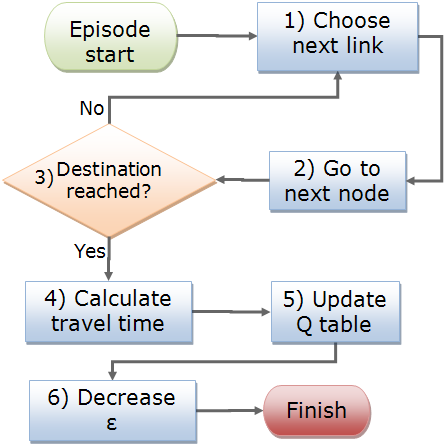
\includegraphics[width=7cm]{img/flowchart3.png}}
    \caption{RL for route choice flowchart}
    \label{fig:flowchart}
\end{figure}

At episode start, all drivers are placed in their origins. At step 1, the driver chooses an outbound link to traverse according to the $\epsilon$-greedy action selection strategy (random action with probability $\epsilon$, best known action with probability $1 - \epsilon$). %TODO increment the road's num-drv

At step 2, the destination node of the chosen link is reached. At step 3, the driver tests whether the node reached is its final destination. If so, the trip ends, otherwise steps 1 to 3 are repeated. At step 4, each driver $i$ calculates its travel time $\att{i}$ experienced on it's route $\route{i}$, given by Eq. \eqref{eq:att}, where $\veh$ is the number of vehicles on link $j$.

\begin{equation}
\label{eq:att}
\att{i} = \sum_{j \in \route{i}} \travTime(\veh)
\end{equation}

Then, at step 5, drivers update their Q-tables according to Eq. \eqref{eq:qlearning}. Finally, at step 6, the exploration coefficient $\epsilon$ is decreased by the multiplicative factor $\lambda$.

\section{Scenarios and metrics}

In the present work two scenarios will be studied. Both are typical commuting scenarios where drivers select a route from their origins to their destinations repeatedly. Drivers going from home to work in the same hour of the day during the workdays is an example of a commuting scenario.

The first scenario is a 6x6 grid, where the convergence and learning properties of the RL approach will be studied. Specifically, two questions are adressed:

\begin{enumerate}
  \item Can drivers learn the routes from origins to destinations without prior knowledge in a nonstationary scenario? As routes are not pre-computed, drivers need to learn how to depart from their origins and arrive at their destinations.
  \item Are drivers improving their performance as the time passes? In this question, we want to assess whether the drivers are reducing their travel times as they gain experience by traveling in the road network repeatedly, that is, if they can take alternative links to a congested one in order to avoid traffic.
\end{enumerate}

The second scenario has 9 possible origin-destination pairs. It is less complex than the 6x6 grid as the number of possible routes between origins and destinations is lower and it is not possible to build routes with loops as there are no returning links. In this scenario, the goal is to compare the RL approach with three methods for route choice.

\subsection{6x6 grid}

This abstract scenario contains 36 nodes connected by 60 links, as shown in Figure \ref{fig:6x6grid}. All links are one-way. Drivers can turn to two directions in each node. From the point of view of route choice, this is a very complex scenario as the number of possible routes between two locations is high and it is possible to build routes with loops, as there is no pre-computation of shortest paths from origins to destinations. For this reason, there is a limit in the number of steps in each episodes: if a driver doesn't find it's destination in 500 steps, the trip is aborted.

\begin{figure}[ht]
    \centerline{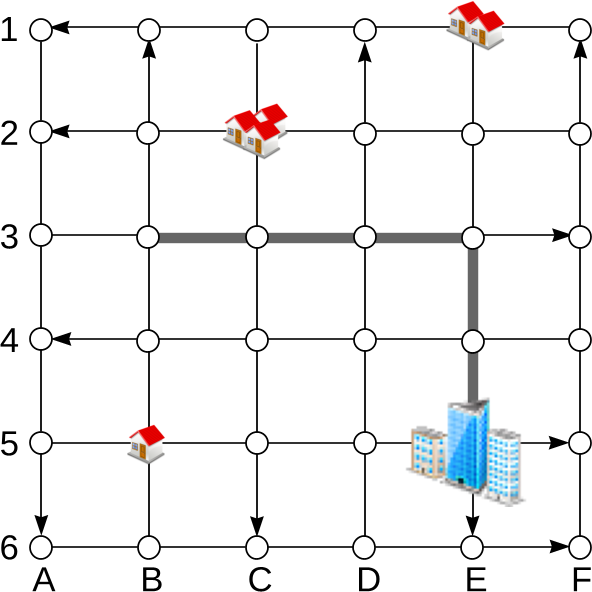
\includegraphics[width=7cm]{img/6x6grid.png}}
    \caption{Abstract grid scenario with the main origins (nodes B5, C2 and E1) and the main destination (node E5). Arrows show the streets' directions. Thicker lines are the main streets.}
    \label{fig:6x6grid}
\end{figure} 

In this scenario, every node is a possible origin or destination, although some nodes have higher probability of being an origin and one node has a high probability of being a destination. Table \ref{tab:odprob} shows the origins and destinations probability distribution, where PO means the probability of the node to be an origin and PD is the probability of the node to be a destination. With this feature, the scenario includes a real-world scenario characteristic: the existance of main residential areas, where commuters depart from (nodes with higher chance of being origins) and a business center, where most commuters arrive in (the node with high chance of being a destination).

{%
%\newcommand{\mc}[3]{\multicolumn{#1}{#2}{#3}}
\begin{table}[ht]
\begin{center}
\begin{tabular}{|l|c|c|} \hline
Node & PO & PD \\ \hline
E5 & 2.67\% & 60\% \\ \hline
B5 & 3\% & 1.15\% \\ \hline
C2 & 4\% & 1.15\% \\ \hline
E1 & 5\% & 1.15\% \\ \hline
Every other node & 2.67\% & 1.15\% \\ \hline
\end{tabular}
\caption{Origins and destinations probability distribution}\label{tab:odprob}
\end{center}
\end{table}
}%
%TODO INSTANTIATE Y AND Z
Regarding the road network capacity, there will be two ``main streets'' with capacity of Y vehicles. The remaining links will be assigned with the capacity of Z vehicles. The main streets are the links between the nodes B3 to E3 and E3 to E4 (thicker lines on Fig. \ref{fig:6x6grid}). With this feature, the abstract 6x6 scenario becomes more realistic, as roads capacities are not homogeneous.

Having the goal of assessing the learning and convergence properties of the RL approach, the following metrics will be evaluated in this scenario:

\begin{itemize}
  \item Number of aborted trips: this metric will assess how many drivers cannot find their destinations within the time limit (500 steps).
  \item Average, maximum and minimum number of steps to reach destination: this metric will assess how many steps drivers are taking to reach their destinations. If drivers take too many steps to finish their trips, this means that they are possibly building routes with loops.
 \item Average, maximum and minimum travel time: this metric will assess how drivers' performance improve with time. More than build a route without loops, drivers need to select links with low occupancy in order to achieve better travel times from their origins to their destinations.
\end{itemize}

\subsection{Nine OD pairs}

The abstract road network used in this scenario is the same studied in \cite{Galib&Moser2011}. It consists on 10 nodes and 24 links, as depicted in Figure \ref{fig:roadnetwork}. All nodes have 3 outbound links, except nodes 8, 9 and 10 which have 2, 1 and 0 outbound links, respectively. Nodes 1, 2 and 3 are the possible origins and nodes 8, 9 and 10 are the possible destinations, resulting in nine possible OD pairs. All possible OD-pairs have uniform probability of being assigned to a driver.

Link's capacities are randomly assigned in the range [130:250] prior to the simulations. The values are persisted from one simulation to another to ensure a correct comparison of different approaches. The same is done for the amount of drivers on each OD pair. There are 1001 drivers on the road network. For Eq. \eqref{eq:tt}, $\fftt$ is set as 5 minutes for all links, $\tau = 1$ and $\beta = 2$ making travel time increase quadratically with the number of drivers.

\begin{figure}[ht]
    \centerline{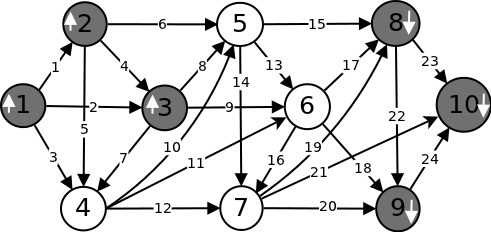
\includegraphics[width=8.5cm]{img/roadnetwork.png}}
    \caption{Road network, the same used by \cite{Galib&Moser2011}. Labels on links are identification numbers, nodes with upward arrows are the origins and downward arrows represent the destinations}
    \label{fig:roadnetwork}
\end{figure}

In this scenario, the RL for route choice approach will be compared with three different route choice methods:

\begin{itemize}
  \item Random: At each step, drivers choose one of the possible outbound links with uniform probability.
  \item Greedy: At initialization, the shortest paths\footnote{It is possible to have more than one shortest path on the road network. Given that link's weights are equal, the shortest paths will be the ones with less links.} for each driver are calculated. At each step, drivers choose one of the possible outbound links with a probability proportional to its capacity. The possible outbound links are the ones that belongs to a shortest path. %TODO mention selfish here
  \item Minority Game: In this approach, drivers use the modified minority game approach proposed by \cite{Galib&Moser2011} to build their routes. A brief description of this approach is given on Section \ref{sec:related}. For a complete description of the approach, it is suggested that readers refer to \cite{Galib&Moser2011}.
\end{itemize}

The comparison of the different route choice methods will be made on metrics regarding reasonable travel times and road network load balance.

\subsubsection{Reasonable travel times:}
In the real world, drivers have an expectation on the trip travel time on the route length, the expected number of drivers in it and the links' capacities. In the present work, for each driver $i$, the expected travel time $\ett{i}$ on his shortest route \optRoute{i} is given by Eq. \eqref{eq:ett}, where $\travTime$ is the travel time function defined in Eq. \eqref{eq:tt} applied to the estimated number of vehicles on the same route ($\expVeh$). This estimation is given by the number of vehicles in driver $i$ OD pair, plus a random number in the range $[-0,05d:0,05d]$, where $d$ is the total number of drivers on the scenario. This ``noise'' is to simulate the effect of each driver ``guessing'' the number of vehicles going to the same destination.

\begin{equation}
\label{eq:ett}
\ett{i} = \sum_{j \in \optRoute{i}}\travTime(\expVeh)
\end{equation}

In order to assess how reasonable are the travel time obtained by drivers, a metric called AED (\underline{a}ctual and \underline{e}xpected travel time \underline{d}ifference) was created. It is given by the difference between actual and expected travel times of each driver. It will be measured in terms of the mean and standard deviation of this difference for all drivers in a given OD pair. The mean will assess whether drivers are arriving at destination within their expectations, on average, and this happens when the metric reaches negative values (actual travel time is lower than expected). The standard deviation will evaluate whether there is a big difference between drivers' AED on the same OD pair, assessing the fairness of the route choice method.

\subsubsection{Road network load balance:}

From a global point of view, it is desired that vehicles get distributed proportionally to the capacity of each link on the network. Road network load balance will be measured in two forms: number of congested links ($n$) and average overload ($o$). Considering $C$ as the set of congested links, these metrics will be measured according to Eq. \eqref{eq:balanceMetrics}, where $\veh_j$ and $\linkCap$ are the number of vehicles and the capacity of link $j$, respectively. 

\begin{equation}
\label{eq:balanceMetrics}
\numCong = |\congRoads| \hspace{1.5cm}  \overLoadFactor = \frac{ \sum_{\substack{j \in \congRoads}} \left(\frac{\veh_j}{\linkCap} -1 \right)}{|C|}
\end{equation}

Both metrics are needed because $n$ alone does not measures how heavy are the links congestions and $o$ does not shows how many links are overloaded. For both ($n$) and ($o$), smaller values means better performance, as less links are congested and the severity of congestions is lower.

\section{Results and discussion}
\label{sec:results}

%TODO will influcence of QL be discussed before the grid scenario?!?

\subsection{Influence of Q-learning parameters}

The following experiments have the goal of assessing the effect of Q-learning parameters, namely the learning rate ($\alpha$) and the discount rate for future rewards ($\gamma$) in both scenarios, so that they can be adjusted accordingly.
%TODO do the alpha-gamma grid tests
\begin{figure}[ht]
  \centering
  \subfigure[]{
    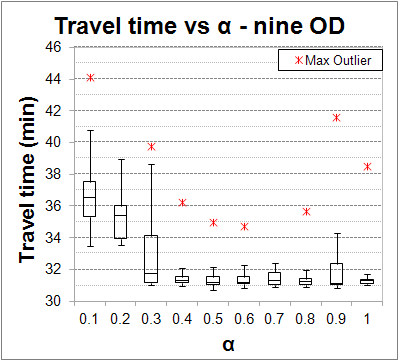
\includegraphics[width=8cm]{img/travelTimeVsAlpha.png}
    \label{fig:travelTimeVsAlpha}
  }
  \subfigure[]{
    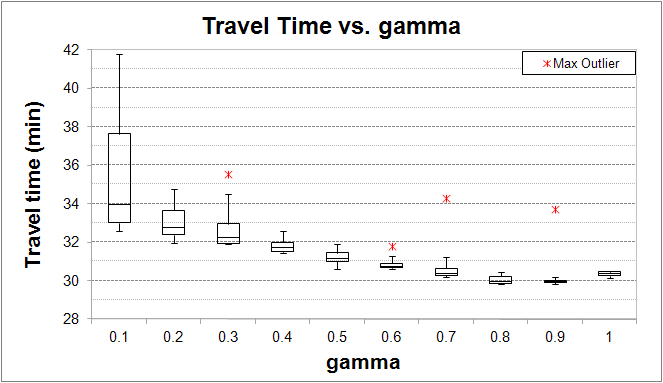
\includegraphics[width=8cm]{img/travelTimeVsGamma.png}
    \label{fig:travelTimeVsGamma}
  }
  \caption{Box-and-whisker charts showing the effect $\alpha$ and $\gamma$ on travel time in the nine OD pair scenario. Each parameter value was tested 10 times.}
  \label{fig:qLearningParams}
\end{figure}

Figure \ref{fig:travelTimeVsAlpha} shows the effect of $\alpha$ and $\gamma$ on drivers' travel time on the nine 0D pairs scenario. The approach performs more robustly for $\alpha$ within the range of 0.4 to 0.8, as the interquartile range is small. For $\alpha = 1.0$ the interquartile range is the smallest, but the maximum outlier is too distant of the upper extreme. This can be due to the nonstationarity of the traffic scenario: if a driver disregards all the previous knowledge, the outcome of a single choice that brought bad results will be fully stored in the Q-table, so that the driver will not try it again (unless the action is tried again by exploration) even if the previous choices resulted in good outcomes. In this kind of nonstationary scenario, a high learning rate can lead to this effect.

Figure \ref{fig:travelTimeVsGamma} shows that a decrease on travel time is observed with the increase of $\gamma$. For $\gamma = 0.9$, the smallest interquartile range and median are observed, showing that the approach performs robustly for this $\gamma$ value.

For the ongoing experiments, the value of $\alpha$ and $\gamma$ will be set as $0.5$ and $0.9$, respectively.

\subsection{6x6 grid scenario}


\subsection{Nine OD pairs scenario}
In this scenario, the goal is to compare the RL approach with the random, greedy and minority game approaches for route choice.

Experiment paramenters are: for Eq. \eqref{eq:tt}, $\fftt$ is set as 5 minutes for all links, $\tau = 1$ and $\beta = 2$ making travel time increase quadratically with the number of drivers. Each run consists of m = 100 learning episodes. The initial and final values for the exploration coefficient are $\epsilon_0 = 1$ and $\epsilon_f = 0.01$, respectively. Then, the value of the multiplicative factor that decreases $\epsilon$ is: $\lambda = \sqrt[100]{\frac{0.01}{1}} = 0.95499$. For the Q-learning update rule (Eq. \eqref{eq:qlearning}), $\alpha = 0.5$ and $\gamma = 0.9$.

The AED metric for each approach is shown on Figure \ref{fig:travelTimeComparison}. 

\begin{figure}[ht]
    \centerline{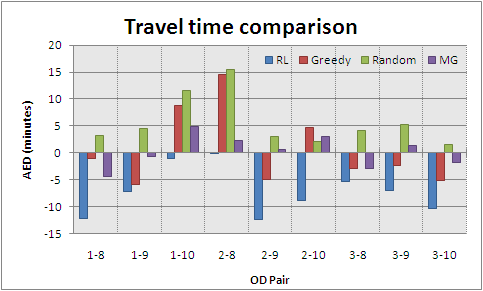
\includegraphics[width=10cm]{img/travelTimeComparison.png}}
    \caption{AED metric comparison for each route choice method. RL and MG are the reinforcement learning and minority game approaches, respectively}
    \label{fig:travelTimeComparison}
\end{figure}

In this metric, the RL approach outperforms the others, achieving reasonable travel times in all OD Pairs. The minority game approach achieves travel times within expectation in 4 OD pairs. On the other OD pairs, the performance is still good, as actual travel times are no longer than 5 minutes beyond the expected, showing a degree of fairness of the approach. With the greedy method, drivers from 5 OD pairs experience travel times within expectation, but especially on OD pairs 1-10 and 2-8, actual travel times are far beyond the expected. The worst approach is the random, in which no drivers achieve reasonable travel times.


\begin{figure}[ht]
  \centering
  \subfigure[]{
    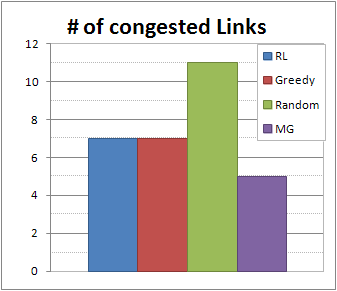
\includegraphics[width=5.8cm]{img/numCongestedRoads.png}
    \label{fig:numCongestedRoads} %TODO num of congested LINK
  }
  \subfigure[]{
    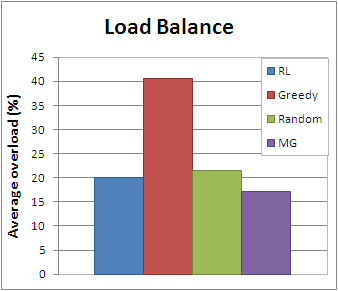
\includegraphics[width=5.8cm]{img/averageOverload.png}
    \label{fig:averageOverload}
  }
  \caption{Load balance evaluation in terms of number of congested links \subref{fig:numCongestedRoads} and the average overload \subref{fig:averageOverload}.}
  \label{fig:loadBalance}
\end{figure}

On the defined load balance evaluation metrics, the minority game based approach achieved the best results. Both the number of congested links and the average overload were the lowest. This means that vehicles were distributed over the network in a proportion that is closer to the links capacity. The RL based approach achieves good results as the average overload shows that none of the seven congested links (out of 24 links) were heavily congested. Both the random and the greedy approach performed poorly, as many links were congested in the random approach and links were heavily congested in the greedy approach.

\section{Conclusions and future work}
\label{sec:conclusions}

In this work we modeled traffic assignment as a reinforcement learning problem and the driver agents were modeled as independent learners.

Regarding the convergence and learning properties, the proposed approach showed itself sensitive to the Q-learning update rule parameters. Specially when the learning rate is lower, the learning does not converge and some drivers don't find routes to their destinations. When these parameters are properly adjusted, the learning converge and drivers improve their performance with time.

In the nine OD pairs scenario, our reinforcement learning for route choice approach was helpful in either individual and global point of view, as drivers achieve reasonable travel times (within expectation) on average, and traffic is distributed over the network, as links does not get heavily congested.

Comparing the RL approach with other route choice methods..... %TODOOOO

The proposed approach has the advantage of making realistic assumptions as it only relies on drivers own experience about the road network (i.e. the experienced travel time), dismissing the use of real-time information and historic data of links. This makes our approach an attractive and feasible alternative to be used on existing navigation systems, as no new technologies are required.

Further investigation can be conducted to evaluate scenarios with heterogeneous drivers. It would be interesting to investigate whether the RL drivers can adapt themselves to the greedy drivers or even the ones using the minority game approach proposed by \cite{Galib&Moser2011}. Future work can also attempt to assess how good it would be for agents when they consider other agents, that is, how good it would be to learn joint actions in this competitive environment.

\section{Acknowledgments}

Authors would like to thank Mr. Syed Galib for clarifying questions on the minority game for route choice approach \cite{Galib&Moser2011} and for providing data for comparison. Both authors are partially supported by CNPq and FAPERGS. %The authors also would like to thank the anonymous reviewers for their suggestions of paper improvements.

\bibliographystyle{splncs03}
\bibliography{references,stringDefs,AB,CD,EG,HJ,KL,MO,OURS,PR,S,TZ} 

\end{document}
